\documentclass[a4paper,twoside]{report}
\usepackage[italian]{babel}
\usepackage[utf8]{inputenc}
\usepackage{amsmath}
\usepackage{amsthm}
\usepackage{amsfonts}
\usepackage{amssymb}
\usepackage{cancel}
\usepackage[margin=1in]{geometry}
\usepackage{hyperref}
\usepackage{bookmark}
\usepackage{setspace}
\usepackage{titlesec}
\usepackage{fancyhdr}
\usepackage{adjustbox}
\usepackage{float}
\usepackage{graphicx}
\usepackage{float}
\usepackage{algpseudocode}
\usepackage[linesnumbered,ruled,vlined]{algorithm2e}
\usepackage{xcolor}
\usepackage{appendix}
\usepackage{xparse}
\usepackage{listings}

\setlength{\parskip}{0pt}
\titlespacing*{\subparagraph}{1em}{0em}{0em} 

\makeatletter
\renewenvironment{abstract}{
    \if@twocolumn
        \section*{\abstractname}%
    \else
        \begin{center}%
            {\bfseries \abstractname\vspace{-.5em}\vspace{\z@}}%
        \end{center}%
        \small
        \begin{quotation}
    \fi}
    {\if@twocolumn\else\end{quotation}\fi}
\makeatother

\let\oldquote\quote
\let\endoldquote\endquote

\RenewDocumentEnvironment{quote}{om}
    {\oldquote}
    {\par\nobreak\smallskip
        \hfill(#2\IfValueT{#1}{~---~#1})\endoldquote 
        \addvspace{\bigskipamount}}

\hypersetup{
    pdfauthor={Luca Facchini},
    pdftitle={Appunti di Sistemi Operativi},
    pdfsubject={Appunti del corso di Sistemi Operativi, tenuto dal prof. Crispo Bruno presso l'Università degli Studi di Trento. Corso seguito nell'anno accademico 2024/2025.},
    pdfkeywords={Sistemi Operativi, Università degli Studi di Trento, Crispo Bruno},
    pdfproducer={LaTeX},
    pdfcreator={pdflatex},
}

\fancypagestyle{chapterInit}{%
    \fancyhf{}
    \renewcommand{\headrulewidth}{0pt}
    \renewcommand{\footrulewidth}{0.4pt}
    \fancyfoot{}
    \fancyfoot[LE,RO]{\thepage}
    \fancyfoot[LO,RE]{``Appunti di Sistemi Operativi" di Luca Facchini}
}
\fancypagestyle{stdPage}{
    \setlength{\headheight}{14.5pt}
    \fancyhead{}
    \fancyhead[LO]{\leftmark}
    \fancyhead[RE]{\rightmark}
    \fancyfoot{}
    \renewcommand{\footrulewidth}{0.4pt}
    \fancyfoot[LE,RO]{\thepage}
    \fancyfoot[LO,RE]{``Appunti di Sistemi Operativi" di Luca Facchini}
}

\fancypagestyle{tocStyle}{
    \pagestyle{stdPage}
    \fancyhead[RE,LO]{}
}
\fancypagestyle{plain}{
    \pagestyle{chapterInit}
}

\graphicspath{{./images/}}

\newtheorem{definition}{Definizione}[chapter]

\title{Appunti di Sistemi Operativi}
\author{Luca Facchini (mat. 245965)}
\date{A.A. 2024/2025}

\begin{document}
    
    % Page numeration to roman
    \pagenumbering{Roman}

    \begin{titlepage}
        \centering  % Center everything on the title page
        {\Huge\textbf{Appunti di Sistemi Operativi}} \\[1cm] % Title
        \vspace{1.5cm}
        
        {\normalsize di: } \\[.3cm]
        {\Large Facchini Luca} \\ % Author name
        \vspace{1.5cm}
        

        {\normalsize Corso tenuto dal prof. Sistemi Operativi} \\[0.3cm] % Course information
        {\large Università degli Studi di Trento} \\[1.5cm]
        
        {\large A.A. 2024/2025} \\[3cm] % Academic year
        
        % Abstract section with spacing control
        \vfill
        \begin{minipage}[t]{0.4\textwidth}
            \begin{flushleft} \normalsize
                \emph{Autore:}\\
                \textsc{Facchini} Luca \\ % Author name
                Mat. 245965 \\
                \vspace{-\baselineskip}
                \begin{tabbing}
                    Email:\= \href{mailto:luca.facchini-1@studenti.unitn.it}{luca.facchini-1@studenti.unitn.it} \\
                        \>  \href{mailto:luca@fc-software.it}{luca@fc-software.it}
                \end{tabbing}
            \end{flushleft}
        \end{minipage}%
        \hfill
        \begin{minipage}[t]{0.4\textwidth}
            \begin{flushleft} \normalsize
                \emph{Corso:}\\
                Sistemi Operativi [146065] \\
                \textsc{CdL}: Laurea Triennale in Informatica \\
                Prof. \textsc{Crispo} Bruno \\
                Email: \href{mailto:bruno.crispo@unitn.it}{bruno.crispo@unitn.it}
            \end{flushleft}
        \end{minipage}
        \vfill
        \begin{abstract}
            Appunti del corso di Sistemi Operativi, tenuto dal prof. Crispo Bruno presso l'Università degli Studi di Trento. Corso seguito nell'anno accademico 2024/2025.\newline
            Dove non specificato diversamente, le immagini e i contenuti sono tratti dalle slide del corso del prof. Crispo Bruno (\href{mailto:bruno.crispo@unitn.it}{bruno.crispo@unitn.it})
        \end{abstract}
        
        % Pushes the content to the center vertically
    \end{titlepage}
    \begingroup
        \pagestyle{tocStyle}
        \addtocontents{toc}{\protect\thispagestyle{tocStyle}}
        \addtocontents{toc}{\protect\pagestyle{tocStyle}}
        \tableofcontents
    \endgroup
    \thispagestyle{tocStyle}
    \pagestyle{stdPage}
    \newpage

    \pagenumbering{arabic}
    
    \chapter{Definizioni e Storia}

    \chapter{Componenti di un sistema operativo}
\label{chap:componentiSO}

Dopo aver definito cosa sia un sistema operativo, vediamo ora quali siano le sue componenti principali, a partire dalla gestione dei processi e della memoria (primaria e secondaria), per poi passare alla gestione dei dell \texttt{I/O} e dei file fino ad arrivare alla protezione, la gestione della rete e l'interprete dei comandi.

\section{Le Componenti in generale}

    \subsubsection{Gestione dei Processi}
        \begin{definition}[Processo]
            Un \textbf{processo} è un programma in esecuzione che necessita di \textbf{risorse} per poter funzionare. Questo inoltre è eseguito in modo \textbf{sequenziale} ed \textbf{una istruzione alla volta}, infine è possibile che un processo sia del \texttt{SO} o dell'utente.
        \end{definition}
        In materia di gestione dei processi il sistema operativo è responsabile nella loro creazione e distruzione, nella loro sospensione e ripresa e deve fornire dei meccanismi per la sincronizzazione e la comunicazione tra i processi stessi.

    \subsubsection{Gestione della memoria primaria}
        \begin{definition}[Memoria primaria]
            La \textbf{memoria primaria} è la memoria principale del computer che conserva dati condivisi dalla \texttt{CPU} e dai dispositivi \texttt{I/O} questa è direttamente accessibile dalla \texttt{CPU}, per essere eseguito un programma deve essere caricato in memoria.
        \end{definition}
        La gestione della memoria primaria richiede la gestione dello spazi di memoria oltre alla decisione su quale processo debba essere caricato in memoria e quale debba essere rimosso. Inoltre il sistema operativo deve fornire dei meccanismi allocare e de-allocare la memoria.

    \subsubsection{Gestione della memoria secondaria}
        \begin{definition}[Memoria secondaria]
            La \textbf{memoria secondaria} è una memoria \textbf{non volatile} ed \textbf{grande} rispetto alla memoria primaria, questa è utilizzata per memorizzare i dati e i programmi in modo \textbf{permanente}.
        \end{definition}
        Questa memoria consiste di uno o più dischi (magnetici) ed il sistema operativo deve fornire dei meccanismi per la gestione dello spazio libero, l'allocazione dello spazio ed lo \textit{scheduling} degli accessi ai dischi.

    \subsubsection{Gestione dell'\texttt{I/O}}
        Il \texttt{SO} nasconde la complessità dell'\texttt{I/O} ai programmi utente, fornendo un'astrazione dell'\texttt{I/O} e fornendo dei meccanismi per: accumulare gli accessi ai dispositivi (\textit{buffering}), fornire una interfaccia generica per i dispositivi e fornire dei \textit{driver} specifici (scritti in \texttt{C}, \texttt{C++} o \textit{assembly}). 

    \subsubsection{Gestione dei file}
        \begin{definition}[File]
            Un \textbf{file} è una sequenza di \textit{byte} memorizzata in un qualsiasi supporto fisico controllato da \textit{driver} del sistema operativo.
        \end{definition}
        Un file è dunque un'astrazione logica per rendere più semplice la memorizzazione e l'uso della memoria \textbf{non volatile}. Il sistema operativo deve fornire dei meccanismi per la creazione, la cancellazione, la lettura e la scrittura di file e \textit{directory} oltre a fornire delle primitive (copia, sposta, rinomina) per la gestione dei file. 

    \subsubsection{Protezione}
        Il sistema operativo deve fornire dei meccanismi per controllare l'accesso a tutte le risorse da parte di processi e utenti, inoltre l'\texttt{SO} è responsabile della definizione di accessi autorizzati e non autorizzati, oltre a definire i controlli necessari ed a fornire dei meccanismi per verificare le politiche di accesso definite.

\section{Come usare i servizi dei sistemi operativi}
    Il sistema operativo metta a disposizione le sue interface tramite delle \textit{system call} che sono delle chiamate a funzione che permettono di accedere ai servizi del sistema operativo precedentemente descritti. Queste chiamate a funzione sono utilizzate per eseguire operazioni che richiedono privilegi di sistema, come ad esempio la gestione dei processi, della memoria, dell'\texttt{I/O} e dei file.
    \subsection{Interprete dei comandi}
        Un esempio di utilizzo delle \textit{system call} è l'interazione con l'interprete dei comandi, che permette di eseguire comandi e programmi tramite una interfaccia testuale. Questo interprete tramuta i comandi in \textit{system call} che vengono poi eseguite dal sistema operativo. Questo permette di creare e gestire processi, gestire \texttt{I/O}, disco, memoria e file oltre alla gestione delle protezione e della rete.\newline
        Nel \texttt{SO} esistono dei comandi predefiniti che possono essere chiamati direttamente per il loro nome, questi sono implementati con una semantica specifica e possono essere utilizzati per eseguire operazioni di base, nel caso di comandi non predefiniti è possibile scrivere dei programmi che vengono eseguiti dall'interprete dei comandi.
    
    \subsection{L'interfaccia grafica}
        Un'altra interfaccia che permette di interagire con il sistema operativo è l'interfaccia grafica, che permette di interagire con il sistema operativo tramite il \textit{mouse} e la tastiera. Questa interfaccia più intuitiva e facile da usare rispetto all'interprete dei comandi, permette di interagire con il \texttt{SO} tramite icone e finestre. Questa interfaccia, anche se più semplice, non è per forza più veloce dell'interprete dei comandi, in quanto l'interfaccia grafica è più lenta e richiede più risorse rispetto all'interprete dei comandi.

    \subsection{\textit{System calls}}
        I processi non usano le \textit{shell} per eseguire le \textit{system call}, ma usano delle \texttt{API} (\textit{Application Programming Interface}) che permettono di accedere ai servizi del sistema operativo. Queste \texttt{API} sono delle librerie di funzioni ad alto livello che permettono di accedere ai servizi del sistema operativo. Queste librerie sono scritte in \texttt{C} o \texttt{C++} e permettono di accedere ai servizi del sistema operativo in modo più semplice e più sicuro rispetto all'uso diretto delle \textit{system call}.
        \paragraph{Esempio di \texttt{API}} Un esempio di \texttt{API} è la \texttt{Win32}, prendiamo in esame la funzione \texttt{ReadFile} che permette di leggere un file:
\begin{lstlisting}[language=C]
    BOOL ReadFile (
        HANDLE file,
        LPVOID buffer,
        DWORD bytes to read,
        LPDWORD bytes read,
        LPOVERLAPPED ovl
    );
\end{lstlisting}
        Questa funzione ritorna un valore booleano che indica se la funzione è andata a buon fine o meno, inoltre questa funzione prende in input il file da leggere, il buffer in cui scrivere i dati letti, il numero di byte da leggere, il numero di byte letti e un puntatore a una struttura \texttt{OVERLAPPED} che permette di specificare un offset per la lettura.
        \subsubsection{Le \texttt{API} nei diversi \texttt{SO}}
            Le 2 \texttt{API} più comuni per Windows sono: \texttt{Win32} e \texttt{Win64} mentre per Linux sono: \texttt{POSIX} (\textit{Portable Operating-System Interface}) che includono le \textit{system call} per tutte le versioni di \texttt{UNIX}, \textit{Linux} e \textit{Mac OS X}, o tutte le distribuzioni \texttt{POSIX}\textit{-compliant}. 
            \paragraph{\textit{Windows} su \textit{Linux}} Per eseguire programmi \textit{Windows} su \textit{Linux} è possibile usare \texttt{Wine} che è un \textit{emulatore} il quale traduce le chiamate \texttt{API} di \textit{Windows} in chiamate \texttt{API} di \textit{Linux} \textit{on-the-fly}, ovvero durante l'esecuzione del programma. Questo permette di eseguire programmi \textit{Windows} su \textit{Linux} senza dover riscrivere il codice del programma.
        
        \subsubsection{Implementazione delle \textit{System Call}}
            Ad ogni \textit{system call} è associato un numero univoco, che permette al sistema operativo di identificare la \textit{system call} richiesta. È compito dell'interfaccia tenere traccia dei numeri associati alle \textit{system call} e di passare i parametri alla \textit{system call} richiesta. Questa interfaccia invoca la \textit{system call} nel \textit{kernel} del sistema operativo, che esegue la \textit{system call} e ritorna il risultato al chiamante. Questo meccanismo permette al chiamante di non dover conoscere i dettagli di implementazione della \textit{system call} ma solo la sua interfaccia.
            \paragraph{Esecuzione delle \textit{system calls}} Per eseguire una \textit{system call} dopo che il processo ha eseguito la chiamata all'interfaccia del \texttt{SO} il quale conoscendo il numero della \textit{system call} controlla dove questa è implementata tramite la \textit{system call table} (una tabella che contiene i puntatori alla implementazione delle \textit{system call}). Una volta trovata la \textit{system call} il \texttt{SO} esegue la \textit{system call} e ritorna il risultato al chiamante.
            \paragraph{Opzioni per il passaggio dei parametri} I parametri di una \textit{system call} possono essere passati in diversi modi. I più comuni sono: passaggio tramite registri, passaggio tramite lo \texttt{stack} e passaggio tramite puntatori. Il passaggio tramite registri è il più veloce ma permette di passare pochi parametri e di piccola dimensione, il passaggio tramite lo \texttt{stack} permette di passare più parametri e di dimensioni maggiori, infine il passaggio tramite puntatori permette di passare parametri di dimensioni maggiori e di passare parametri complessi, ma và passata una tabella di parametri che deve essete passata tramite \texttt{stack} o registri.
                \subparagraph{Parametri tramite \texttt{stack}} Il passaggio dei parametri tramite \texttt{stack} avviene in questo modo:
                    \begin{enumerate}
                        \item[1-3] Salvataggio parametri sullo \texttt{stack}
                        \item[4] Chiamata della funzione di libreria
                        \item[5] Caricamento del numero della \textit{system call} su un registro \texttt{Rx}
                        \item[6] Esecuzione \texttt{TRAP} (Passaggio in \textit{kernel mode})
                        \item[7-8] Esecuzione della \textit{system call}
                        \item[9] Ritorno al chiamante 
                        \item[10-11] Ritorno al codice utente ed incremento dello \texttt{stack pointer} 
                    \end{enumerate}
                    \begin{figure}[H]
                        \centering
                        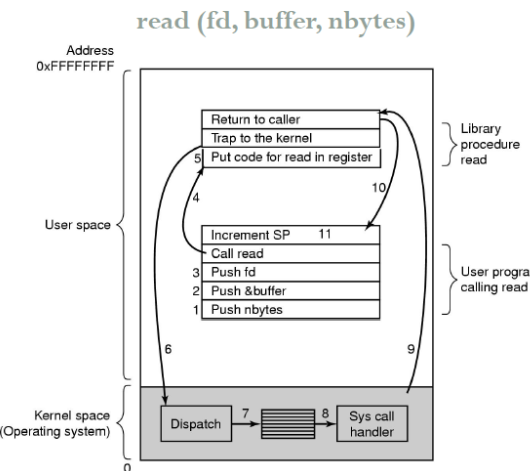
\includegraphics[width=0.3\textwidth]{images/02/stackCall.png}
                        \caption{Passaggio dei parametri tramite \texttt{stack}}
                    \end{figure}
                \subparagraph{Passaggio di parametri tramite tabella} 
                    Come anticipato il passaggio di parametri tramite tabella viene utilizzato per passare parametri complessi o di dimensioni maggiori andando a passare un puntatore alla tabella che contiene i parametri. Questo metodo permette di passare un numero maggiore di parametri e di dimensioni maggiori in quanto i parametri sono passati per riferimento alla memoria primaria.
                    \begin{figure}[H]
                        \centering
                        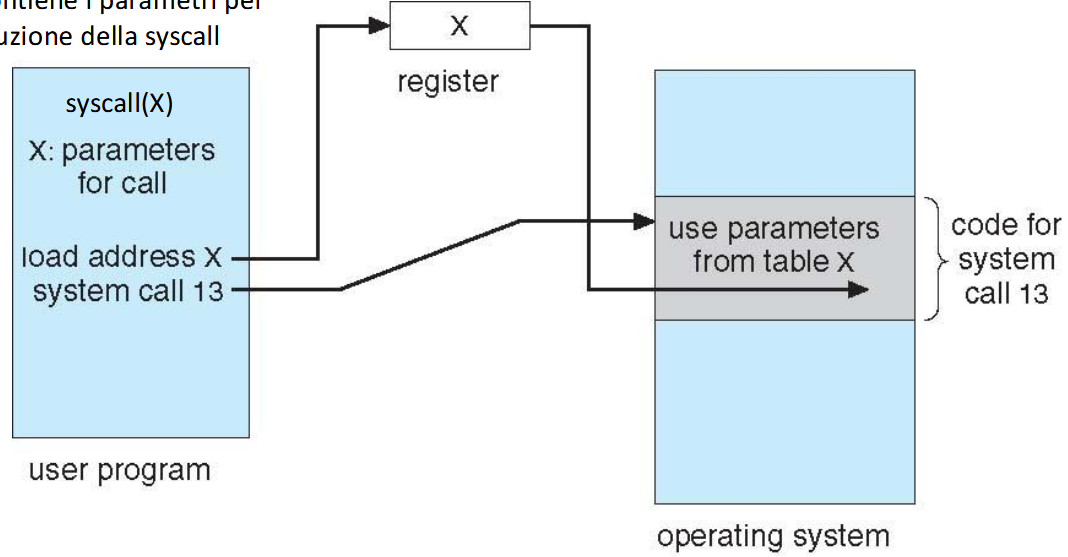
\includegraphics[width=0.3\textwidth]{images/02/tabCall.png}
                        \caption{Passaggio dei parametri tramite tabella}
                    \end{figure}
                    
    \chapter{Architettura di un Sistema Operativo}

In un sistema operativo è molto importante separare le \textit{policy} dai \textit{meccanismi}. I meccanismi sono le funzionalità che il sistema operativo mette a disposizione, mentre le \textit{policy} sono le regole che il sistema operativo segue per decidere come utilizzare i meccanismi.

\paragraph{Principi di progettazione} Il principio di progettazione di un sistema operativo è quello di \texttt{KISS} (\textit{Keep It Small and Simple}) usato per ottimizzare al meglio le \textit{performance} implementando solo lo stretto necessario. Altro principio è il \texttt{POLP} (\textit{Principle of Least Privilege}), ovvero dare il minimo dei privilegi necessari ad ogni componente per svolgere il proprio compito. Quest'ultimo principio è molto importante per garantire affidabilità e sicurezza.

\section{Tipi di architetture}
    \subsubsection{Sistemi monoblocco}
        Nei sistemi monoblocco non è presente una gerarchia tra i vari livelli del sistema operativo. Questo tipo di architettura è molto semplice e consiste in un unico strato \textit{software} tra l'utente ed l'\textit{hardware} del sistema. Le componenti sono dunque tutte allo stesso livello permettendo una comunicazione diretta tra l'utente e l'\textit{hardware}. Questo tipo di architettura è molto semplice e veloce, ma il codice risulta interamente dipendente dall'architettura ed è distribuito su tutto il sistema operativo. Inoltre per testare ed eseguire il \textit{debugging} di un singolo componente è necessario analizzare l'intero sistema operativo.
    \subsubsection{Sistemi a struttura semplice}
        Nei sistemi a struttura semplice è presente una piccola gerarchia, molto flessibile, tra i vari livelli del sistema operativo. Questo tipo di architettura mira ad una riduzione dei costi di sviluppo ed di manutenzione del sistema operativo. Non avendo una struttura ben definita, i componenti possono comunicare tra loro in modo diretto. Questo tipo di architettura è molto flessibile e permette di avere un sistema operativo molto piccolo e veloce come \texttt{MS-DOS} o \texttt{UNIX} originale.
        \paragraph{\texttt{MS-DOS}} Il sistema operativo \texttt{MS-DOS} è un sistema operativo a struttura semplice, molto piccolo e veloce. Questo sistema operativo è pensato per fornire il maggior numero di funzionalità in uno spazio ridotto. Infatti non sussistono suddivisioni in moduli, ed le interfacce e livelli non sono ben definiti. È infatti possibile accedere direttamente alle \textit{routine} del sistema operativo ed non è prevista la \textit{dual mode}.
        \paragraph{\texttt{UNIX} (Originale)} Struttura semplice limitata dalle poche funzionalità disponibili all'epoca in materia di \textit{hardware}, con un \textit{kernel} molto piccolo e veloce il quale scopo è risiedere tra l'interfaccia delle \textit{system call} e l'\textit{hardware}. Questo sistema operativo è stato progettato per essere molto flessibile e fornisce: \textit{File System}, \textit{Scheduling} della \texttt{CPU}, gestione della memoria e molto altro.
        \begin{figure}[H]
            \centering
            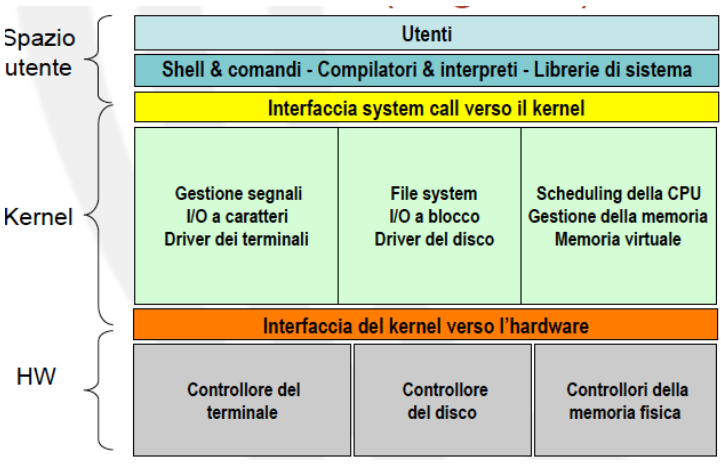
\includegraphics[width=0.6\textwidth]{03/unixOriginal.png}
            \caption{Struttura di \texttt{UNIX} originale}
        \end{figure}
    \subsubsection{Sistema a livelli}
        Nei sistemi operativi organizzati a livelli gerarchici l'interfaccia utente risiede al livello più altro mentre l'\textit{hardware} dal lato opposto. Ogni livello intermedio può solo usare funzioni fornite dal livello inferiore ed offrire funzionalità al livello superiore. Principale vantaggio di questa architettura è la modularità, infatti ogni livello può essere sviluppato e testato indipendentemente dagli altri. Questo tipo di architettura, d'altronde non è priva di svantaggi, infatti diventa difficile definire in modo approssimato gli strati, l'efficienza decresce in quanto ogni singolo strato aggiunge un costo di \textit{overhead} ed le funzionalità dipendenti dal'\textit{hardware} sono sparse su più livelli.
        \paragraph{\texttt{THE}} Il sistema operativo \texttt{THE} è un sistema d'uso accademico ed è il primo sistema operativo a struttura a livelli. Questo \texttt{SO} consiste in un insieme di processo che cooperano tra di loro usando la tecnica dei ``semafori'' per la sincronizzazione. \begin{figure}[H]
            \centering
            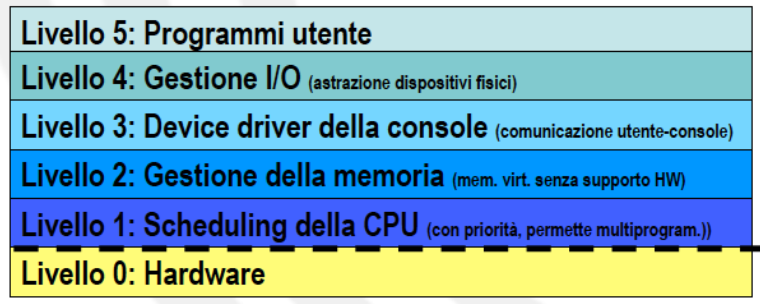
\includegraphics[width=0.4\textwidth]{03/the.png}
            \caption{Struttura di \texttt{THE}}
        \end{figure}
    
    \subsubsection{Sistemi basati su \textit{Kernel}}
        I sistemi di questo genere hanno due soli livelli: i servizi \textit{kernel} e quelli non-\textit{kernel} (o \textit{utente}). Il \textit{file system} è un esempio di servizio non-\textit{kernel}. Questo tipo di architettura è molto diffuso in quanto il ridotto e ben definito numero di livelli ne permette una facile implementazione e manutenzione, spesso però questo sistema può risultare troppo rigido e non adatto a tutti i tipi di applicazioni, oltre alla totale assenza di regole organizzative per le parti del \texttt{SO} al di fuori del \textit{kernel}.
    \subsubsection{\textit{Micro-kenrel}} 
        Questo tipo di \textit{kernel} è molto piccolo e fornisce solo i servizi essenziali per il funzionamento del sistema operativo. Tutte le altre funzionalità sono implementate come processi utente. Un esempio di ciò è \texttt{seL4} un \textit{kernel} \textit{open source} che implementa un \textit{micro-kernel} e fornisce un'interfaccia per la gestione della memoria, dei processi e della comunicazione tra processi. \texttt{SeL4} è matematicamente verificato e privo di bug rispetto alle sue specifiche di forte sicurezza 
    \subsubsection{\textit{Virtual Machine}}
        L'architettura a \texttt{VM} è una estremizzazione dell'approccio a più livelli di \texttt{IBM} (1972), questo è pensato per offrire un sistema di \textit{timesharing} ``multiplo'' dove il sistema operativo viene eseguito su una \texttt{VM} ed questa dà illusione di processi multipli, ma nella realtà ognuno di questi è in esecuzione sul proprio \texttt{HW}. In questo paradigma sono possibili più \texttt{SO} in una unica macchina. 
        \begin{figure}[H]
            \centering
            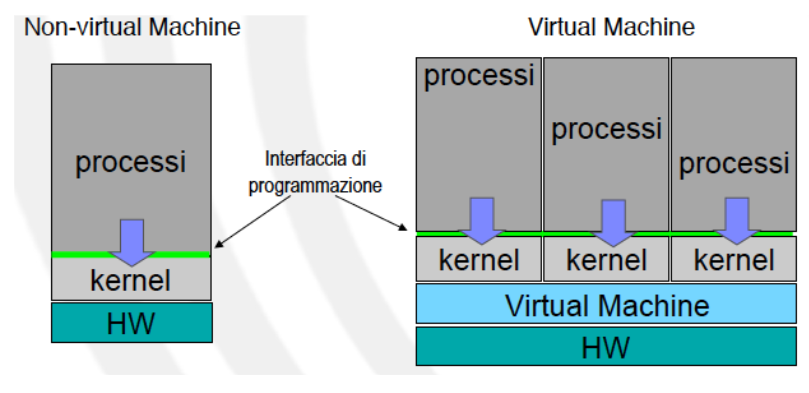
\includegraphics[width=0.4\textwidth]{03/diffVmNoVm.png}
            \caption{Differenze tra una macchina senza e con \texttt{VM}}
        \end{figure}
        Come è possibile notare ogni singolo processo è separato ed possiede il proprio \textit{kernel}. Vengono quindi separata la multiprogrammazione ed la presentazione.
        \paragraph{Tipo di \textit{Hypervisor}}
            \begin{itemize}
                \item \textbf{Tipo 1} (\textit{Bare Metal}): Questo tipo di \textit{Hypervisor} è installato direttamente sul'\textit{hardware} e non necessita di un sistema operativo ospite. Questo tipo di \textit{Hypervisor} è molto veloce e sicuro, ma è molto complesso da installare e configurare.
                \item \textbf{Tipo 2} (\textit{Hosted}): Questo tipo di \textit{Hypervisor} è installato sopra un sistema operativo ospite. Questo tipo di \textit{Hypervisor} è molto più semplice da installare e configurare rispetto al tipo 1, ma è più lento e meno sicuro, inoltre è possibile avere problemi di compatibilità tra il sistema operativo ospite e il \textit{Hypervisor}.
            \end{itemize}
        \paragraph{\textit{Monolithic} vs \textit{Micro-kernel} \texttt{VM}}
            Prima di fare una distinzione tra i due tipi di \texttt{VM} è necessario dire che entrambi rientrano nel tipo 1 di \textit{Hypervisor} e dunque tutti i \texttt{SO} sono eseguiti direttamente sul'\textit{hardware} virtualizzato.
            \begin{itemize}
                \item \textbf{\textit{Monolithic}}: Questo tipo di \texttt{VM} è molto simile ad un sistema operativo tradizionale, infatti ogni \textit{VM} è un processo separato che esegue il proprio \textit{kernel}. Questo tipo di \texttt{VM} è molto veloce, ma è molto complesso da implementare e mantenere.
                \item \textbf{\textit{Micro-kernel}}: Questo tipo di \texttt{VM} è molto simile ad un sistema operativo a \textit{micro-kernel}, infatti il \textit{kernel} della \texttt{VM} fornisce solo i servizi essenziali per il funzionamento del sistema operativo. Tutte le altre funzionalità sono implementate come processi utente. Questo tipo di \texttt{VM} è molto più semplice da implementare e mantenere rispetto al tipo 1, ma è più lento e meno sicuro.
            \end{itemize}
        \paragraph{Vantaggi - Svantaggi}
            Principale vantaggio di questo tipo di architettura è la completa protezione del sistema, infatti ogni \texttt{SO} è separato e non può accedere alle risorse degli altri \texttt{SO}. Inoltre è possibile avere più \texttt{SO} in una sola macchina andando ad ottimizzare le risorse e ridurre i costi di sviluppo di un sistema operativo, oltre ad aumentare la portabilità delle applicazioni. Principale svantaggio riguardano le prestazioni del sistema, infatti ogni \texttt{SO} è eseguito su una \texttt{VM} e questo può portare ad un aumento dei tempi di esecuzione delle applicazioni. Inoltre è necessario avere gestire una \textit{dual-mode} virtuale e non è possibile avere un sistema operativo in tempo reale, inoltre il fatto che una \texttt{VM} non possa accedere alle altre \texttt{VM} può portare ad un aumento dei costi di sviluppo e manutenzione del sistema.
    \subsubsection{Sistemi \textit{client-server}}
        Poco diffusi ai giorni nostri, i sistemi \textit{client-server} sono basati su un'architettura a due livelli: il \textit{client} e il \textit{server}. Questo sistema di basa sull'idea che il codice del sistema operativo vada portato sul livello superiore (il \textit{client}) e il \textit{server} rimanga molto piccolo e veloce andando solo a fornire i servizi essenziali per il funzionamento del sistema operativo ed la comunicazione tra il \textit{client} e l'\textit{hardware}. Questo tipo di architettura si presta bene per sistemi distribuiti.
\section{Implementazione di un \texttt{SO}}
    I sistemi operativi sono tradizionalmente scritti in linguaggio \textit{assembler} anche se è possibile scriverli in linguaggi di alto livello, come \texttt{C} o \texttt{C++}. La scrittura di un sistema operativo in linguaggio di alto livello permette di avere una implementazione molto rapida oltre ad aumentarne la compattezza e la mantienebilità. Inoltre è possibile avere una maggiore portabilità del sistema operativo, in quanto è possibile compilare il codice sorgente su più architetture. Tuttavia la scrittura di un sistema operativo in linguaggio di alto livello può portare ad un aumento dei tempi di esecuzione delle applicazioni e ad un aumento dei costi di sviluppo e manutenzione del sistema operativo. 
    \chapter{Processi e \textit{Thread}}

In questo capitolo vedremo cosa sono i processi e i \textit{thread} capendone le differenze e le somiglianze, vedremo come vengono gestiti e come vengono eseguiti. Infine vedremo come vengono gestiti i processi dal sistema operativo e come vengono eseguiti i processi dal sistema operativo.

\section{Processi}
    Un processo è l'istanza di un programma in esecuzione, quando il programma viene eseguito e quindi caricato nella memoria primaria (\texttt{RAM}) diventa un processo. Mentre un programma è la parte statica di un software, il processo è la parte dinamica. Un processo viene eseguito in maniera sequenziale, ovvero un'istruzione alla volta, ma nei sistemi operativi moderni un processo può essere eseguito in maniera concorrente, ovvero più processi possono essere eseguiti in parallelo.
    \subsubsection{Immagine in memoria}
        Un processo quando viene caricato in memoria viene caricato in una zona di memoria chiamata \textit{spazio degli indirizzi} (\textit{address space}). Questo spazio è diviso in varie sezioni (da indirizzi alti ad indirizzi bassi):
        \begin{itemize}
            \item \textbf{Dati}: contiene le variabili globali e statiche del programma.
            \item \textbf{\textit{Stack}}: contiene le variabili locali e i parametri delle funzioni.
            \item eventuale memoria dinamica allocata durante l'esecuzione.
            \item \textbf{\textit{Heap}}: contiene la memoria dinamica allocata durante
            \item \textbf{Codice}: contiene il codice del programma.
            \item \textbf{Attributi del processo}: contiene informazioni sul processo.
        \end{itemize}
    \subsection{Stato di un processo}
        Un processo durante la sua creazione ed esecuzione può trovarsi in diversi stati:
        \begin{itemize}
            \item \textbf{Nuovo}: il processo è stato creato ma non è ancora in esecuzione.
            \item \textbf{Pronto}: il processo è pronto per essere eseguito, ma non è ancora in esecuzione. (oppure è stato messo in attesa dalla \texttt{CPU}).
            \item \textbf{In esecuzione}: il processo è in esecuzione sulla \texttt{CPU}.
            \item \textbf{In attesa}: il processo è in attesa di un evento (es. \texttt{I/O}).
            \item \textbf{Terminato}: il processo è terminato.
        \end{itemize}
        Per la gestione di questi stati il sistema operativo usa un \textit{dispatcher} il quale compito è quello di passare tra i processi e cambiare il loro stato. Per questo motivo il \textit{dispatcher} è chiamato anche \textit{scheduler}.
        \subsubsection{\textit{Scheduling}}
        \label{sec:scheduling04}
            Lo \textit{scheduling} è il processo di selezione del processo da eseguire sulla \texttt{CPU}. Esistono vari tipi di \textit{scheduler}:
            \begin{itemize}
                \item \textbf{\textit{Long time scheduler}}: decide quali processi devono essere caricati in memoria. (Nella coda dei processi pronti).
                \item \textbf{\textit{Short time scheduler}}: decide quale processo deve essere eseguito sulla \texttt{CPU}. (Seleziona i processi dalla coda dei processi pronti).
            \end{itemize}
            Mentre lo \textit{short-term} scheduler è un processo molto veloce in quanto viene chiamato molto spesso (ogni $10-100 ms$), il \textit{long-term} scheduler è un processo più lento in quanto viene chiamato molto raramente (ogni $1-10 s$ o anche di più), questo però è responsabile del grado di multiprogrammazione del sistema. 
            \paragraph{Accantonamento}
                L'accantonamento è il processo per il quale i processi pronti ad essere eseguiti vengono messi in una coda di attesa. Quando la \texttt{CPU} è pronta per eseguire un processo, il processo viene preso dalla coda e viene eseguito, nel caso nel quale il processo richieda un'operazione di \texttt{I/O} il processo viene messo in richiesta ed quando l'operazione di \texttt{I/O} (caratterizzata a sua volta da una coda per ogni dispositivo connesso) è completata il processo viene rimesso nella coda dei processi pronti.\newline 
                Può anche succedere che il tempo per l'esecuzione di un processo sia scaduto, in questo caso il processo viene rimesso nella coda dei processi pronti. Se poi il processo generi dei processi figli, questi dopo la loro inizializzazione vengono messi nella coda dei processi pronti e vengono eseguiti, se il padre necessita che il processo figlio termini prima di lui, il padre viene messo in attesa che il figlio termini, altrimenti anche il padre viene messo nella coda dei processi pronti. Infine se un processo necessita di un segnale da parte di un altro processo, il processo viene messo in attesa finché non riceve il segnale (dal sistema o da un altro processo).
            \paragraph{\texttt{I/O} vs \texttt{CPU} \textit{bound}}
                Un processo può essere \texttt{I/O} bound o \texttt{CPU} \textit{bound}. Un processo \texttt{I/O} \textit{bound} è un processo che richiede molte operazioni di \texttt{I/O} e poche operazioni sulla \texttt{CPU}, mentre un processo \texttt{CPU} \textit{bound} è un processo che richiede molte operazioni sulla \texttt{CPU} e poche operazioni di \texttt{I/O}. Non è possibile stabilire a priori se un processo è \texttt{I/O} \textit{bound} o \texttt{CPU} \textit{bound}, ma è possibile stabilirlo solo durante l'esecuzione del processo analizzando quanta \texttt{CPU} usa e se richiede molte operazioni di \texttt{I/O}, sulla base di questo il processo viene classificato come \texttt{I/O} \textit{bound} o \texttt{CPU} \textit{bound}.
        \subsubsection{Operazione di \textit{dispatch}}
            Quando si deve passare da un processo ad un altro si deve fare un'operazione di \textit{dispatch}. Questa operazione consiste nel:
            \begin{enumerate}
                \item Cambiare il contesto (salvare lo stato del processo corrente (\texttt{PCB}) e caricare lo stato del processo successivo (\texttt{PCB})).
                \item Passare alla modalità utente (quando viene eseguito il \textit{context switch} il sistema operativo è in modalità \textit{kernel}, mentre il processo deve essere eseguito in modalità utente).
                \item Salto alla prossima istruzione da eseguire del processo successivo.
            \end{enumerate}
            Questa operazione è molto costosa in termini di tempo, in particolare l'operazione di \textit{context switch} richiede risorse che rallentano il sistema senza eseguire nessuna operazione utile, la durata di ciò è strettamente dipendente dall'architettura del processore e dal sistema operativo.
    \subsection{Operazioni sui processi}
        Nella quasi totalità dei sistemi operativi moderni è possibile eseguire più processi in parallelo, per fare ciò il sistema operativo deve fornire delle operazioni per la gestione dei processi oltre ad un modo per l'identificazione dei processi. Di seguito vediamo quali sono le operazioni possibili sui processi.
        \subsubsection{Creazione di un processo}
            Un processo, come già detto, può creare altri processi, questi processi creati sono detti processi figli. Un processo padre può creare più processi figli, questi processi figli possono creare a loro volta altri processi figli e così via. Ai processi normalmente viene associato un \textit{PID} (\textit{Process IDentifier}) che è un numero univoco che identifica il processo all'interno del sistema operativo. \newline
            Il processo figlio può ottenere le risorse necessarie per la sua esecuzione in due modi:
            \begin{itemize}
                \item Ereditando le risorse del processo padre (\textit{sharing})
                \item Ottenendo nuove risorse dal sistema operativo (\textit{partitioning})
            \end{itemize}
            Inoltre il processo figlio può essere eseguito in parallelo in maniera sincrona rispetto al processo padre (il processo padre aspetta che il processo figlio termini) o asincrona (il processo figlio viene eseguito in parallelo al processo padre).
            \paragraph{Nei sistemi \texttt{UNIX}} Nei sistemi \texttt{UNIX} esistono diverse \textit{system call} per la creazione di processi, la principale è \texttt{fork()} che crea un processo figlio identico al processo padre, la differenza tra i due processi è il \textit{PID} e il \textit{PPID} (\textit{Parent Process IDentifier}). Il processo figlio eredita tutte le risorse del processo padre, inoltre il processo figlio può modificare le risorse ereditate dal processo padre. Altra chiamata di sistema è \texttt{exec()} che permette di caricare un nuovo programma in un processo figlio, in questo caso il programma tra il processo padre e il processo figlio è differente. Infine la chiamata di sistema \texttt{wait()} permette l'esecuzione sincrona di un processo figlio rispetto al processo padre.
        \subsubsection{Terminazione di un processo}
            Un processo può terminare in tre modi:
            \begin{itemize}
                \item \textbf{Normalmente}: il processo termina la sua esecuzione invocando la \textit{system call} \texttt{exit()} (con eventualmente un codice di uscita).
                \item \textbf{Forzatamente dal processo padre}: il processo padre può terminare il processo figlio invocando la \textit{system call} \texttt{kill()}, oppure nel caso di un eccessivo uso di risorse, oppure a sua volta il processo padre termina anormalmente.
                \item \textbf{Forzatamente dal sistema operativo}: il sistema operativo può terminare un processo nel caso di un errore di esecuzione, oppure nel caso nel quale l'utente chiuda l'applicazione.
            \end{itemize}
            Nota come nel primo caso non sia esclusa la possibilità che il processo termini in maniera anomala, ad esempio per un errore di esecuzione gestito dal processo stesso, infatti quando il codice di uscita è diverso da \texttt{0} si intende che il processo è terminato in maniera anomala, ogni codice diverso da \texttt{0} ha un significato diverso.\newline
            Quando un processo termina il sistema operativo si occupa di liberare le risorse utilizzate dal processo come la memoria allocata, i file aperti, le connessioni di rete, o altre risorse.
    \subsection{Gestione dei processi del \texttt{SO}}
        Di fatto il sistema operativo non è altro che un programma a tutti gli effetti, e dunque la sua esecuzione è un processo come un altro. Questo non significa però che il sistema operativo non essere gestito separatamente dagli altri processi, infetti esistono diverse opzioni l'esecuzione del \textit{kernel}:
        \begin{itemize}
            \item Il \textit{kernel} viene eseguito completamente in maniera separata dagli altri processi.
            \item Il \textit{kernel} viene eseguito all'interno di un processo utente.
            \item Il \textit{kernel} viene eseguito come un processo separato.
        \end{itemize}
        \paragraph{\textit{Kernel} separato} In questo caso il \textit{kernel} è eseguito al di fuori degli altri processi, questo gli permette di avere uno spazio in memoria ben definito e riservato oltre ad avere il totale controllo del sistema ed a essere eseguito in modalità \textit{kernel} (ovvero con privilegi elevati). I processi sono dunque solo propri all'utente ed un processo non potrà mai essere eseguito in modalità \textit{kernel}.
        \paragraph{\textit{Kernel} nel processo utente} In questo caso il \textit{kernel} è eseguito all'interno di un processo utente, questo permette ai programmi utente di chiamare qualunque servizio del sistema operativo, ma tramite una modalità protetta (\textit{kernel mode}) che permette al sistema operativo di controllare le chiamate e di evitare che un processo utente possa fare danni al sistema. Dato che il \textit{kernel} è un processo a tutti gli effetti la sua immagine in memoria sarà composta dal ``\textit{kernel stack}'' per la gestione delle chiamate di sistema e dal ``\textit{kernel code}'' che consiste nei dati e codice del \texttt{SO} condiviso tra tutti i processi.\newline
        Questo approccio porta ad una riduzione del tempo di \textit{context switch} in quanto è necessario solo la \textit{mode switch} e non l'intero \textit{context switch} lasciando però intatte le possibilità di riattivazione del processo utente o di eseguire un altro processo eseguendo un \textit{context switch} completo.
        \paragraph{\textit{Kernel} come processo separato} In questo caso ogni servizio del sistema operativo è eseguito come un processo separato in modalità protetta. L'unica parte del \textit{kernel} che deve essere eseguita separatamente è lo \textit{scheduler} in quanto deve essere eseguito in modalità \textit{kernel}. Questo approccio è molto vantaggioso per sistemi multiprocessore in quanto permette di eseguire i servizi del sistema operativo in parallelo ed in un processore designato.
\section{\textit{Thread}}
    Un \textit{thread} è l'unità di base d'uso della \texttt{CPU}, un processo può contenere uno o più \textit{thread} che condividono lo stesso codice, dati e file aperti, ma ognuno ha un suo \textit{stack}, lo stato del \textit{program counter} e dei registri ed un numero identificativo.\newline
    Dunque le risorse e lo spazio di indirizzamento sono propri del processo, mentre lo stato della \texttt{CPU} è proprio del \textit{thread} assieme al \textit{program counter} e ai registri.\newline
    Classicamente un processo è composto da un solo \textit{thread}, la capacità di avere più \textit{thread} in un processo è chiamata \textit{multithreading}. Questo permette di avere un processo con più \textit{thread} separando il flusso di esecuzione e lo spazio di indirizzamento, ma condividendo le risorse del processo. 
    \paragraph{Vantaggi}
        I vantaggi del \textit{multithreading} sono:
        \begin{itemize}
            \item \textbf{Risposta più veloce}: Se sono necessari molti calcoli o operazioni di \texttt{I/O} è possibile eseguire queste operazioni in parallelo.
            \item \textbf{Condivisione delle risorse}: I \textit{thread} possono condividere le risorse del processo, mentre processi separati devono usare meccanismi di comunicazione.
            \item \textbf{Economia}: Creare un \textit{thread} è più veloce e meno costoso di creare un processo.
            \item \textbf{Scalabilità}: I \textit{thread} possono essere eseguiti in parallelo su più processori o su più core.
        \end{itemize}
    \subsection{Implementazione dei \textit{thread}}
        Vediamo ora come sono implementati i \textit{thread} nei sistemi operativi.
        \subsubsection{Stato dei \textit{thread}}
            Un \textit{thread}, come un processo, può trovarsi in diversi stati:
            \begin{itemize}
                \item \textbf{Pronto}: il \textit{thread} è pronto per essere eseguito.
                \item \textbf{In esecuzione}: il \textit{thread} è in esecuzione sulla \texttt{CPU}.
                \item \textbf{In attesa}: il \textit{thread} è in attesa di un evento.
            \end{itemize}
            Un \textit{thread} può essere in uno di questi stati, ma il processo può non essere nello stesso stato di un \textit{thread} in quanto un processo può contenere più \textit{thread} e quindi un processo può essere in uno stato diverso da quello dei suoi \textit{thread}.\newline
            Un classico problema degli stati dei \textit{thread} è la questione di cosa fare quando un \textit{thread} è in attesa di un evento, questa ``attesa'' deve bloccare l'intero processo o solo il \textit{thread} in attesa? Ciò dipende dall'implementazione dei \textit{thread} nel sistema operativo.
        \subsubsection{Implementazione dei \textit{thread}}
            Esistono due principali implementazioni dei \textit{thread}:
            \begin{itemize}
                \item \textbf{\textit{User-level threads}}: I \textit{thread} sono implementati a livello utente, il sistema operativo non è a conoscenza dei \textit{thread} e non li gestisce. Le funzionalità sono implementate in una libreria che gestisce i \textit{thread} e le chiamate di sistema.
                \item \textbf{\textit{Kernel-level threads}}: I \textit{thread} sono implementati a livello del \textit{kernel}, il sistema operativo è a conoscenza dei \textit{thread} e li gestisce. 
                \item \textbf{\textit{Hybrid threads}}: I \textit{thread} sono implementati a livello del \textit{kernel}, ma il sistema operativo permette di creare \textit{thread} a livello utente. (es. \texttt{SOLARIS})
            \end{itemize}
            \paragraph{\textit{User-level threads}} Se si opta per l'implementazione dei \textit{thread} a livello utente, il sistema operativo non è a conoscenza dei \textit{thread} e non li gestisce e dunque non è necessario passare in modalità \textit{kernel} per la gestione dei \textit{thread} risparmiando due \textit{context switch}. Ogni applicazione deve però implementate lo \textit{scheduler} dei \textit{thread} e la gestione degli stati dei \textit{thread}. Quanto detto garantisce una maggiore portabilità delle applicazioni senza dover riscrivere il codice per ogni sistema operativo, ma allo stesso tempo non permette di sfruttare appieno le potenzialità del sistema operativo. Se però un \textit{thread} necessita di un'operazione di \texttt{I/O} o di un'operazione che richiede l'intervento del sistema operativo, tutti i \textit{thread} del processo vengono bloccati in quanto il sistema operativo non è a conoscenza dei \textit{thread} e non può gestire i \textit{thread} in maniera indipendente. (es. \textit{Green threads (\texttt{JDK1.1})}, \texttt{GNU} \textit{Portable Threads}, \texttt{POSIX} \textit{Pthreads})
            \paragraph{\textit{Kernel-level threads}} Se si opta per l'implementazione dei \textit{thread} a livello del \textit{kernel}, il sistema operativo è a conoscenza dei \textit{thread} e li gestisce, dunque il sistema operativo può gestire i \textit{thread} in maniera indipendente e può sfruttare appieno le potenzialità del sistema operativo. Ogni \textit{thread} è un processo a tutti gli effetti, dunque ogni \textit{thread} ha il proprio \textit{PCB} e il proprio spazio di indirizzamento. Questo permette di sfruttare appieno le potenzialità del sistema operativo, ma allo stesso tempo richiede due \textit{context switch} per passare da un \textit{thread} all'altro. (es. \texttt{Windows}, \texttt{Linux}, \textit{Native Threads (\texttt{JDK1.2})})
            \paragraph{\textit{Hybrid threads}} Se si opta per l'implementazione dei \textit{thread} ibridi, il sistema operativo permette di creare \textit{thread} a livello utente, ma i \textit{thread} sono implementati a livello del \textit{kernel}. Questo permette di sfruttare appieno le potenzialità del sistema operativo, ma allo stesso tempo permette di creare \textit{thread} a livello utente. (es. \texttt{SOLARIS})
    \subsection{Esempio di libreria - \texttt{pthreads}}
        Nel caso di implementazione dei \textit{thread} a livello utente, il sistema operativo non è a conoscenza dei \textit{thread} e dunque non li gestisce, ma è necessario utilizzare una libreria che gestisca i \textit{thread}. Un esempio di libreria per la gestione dei \textit{thread} è \texttt{pthreads} (\texttt{POSIX} \textit{Threads}).\newline
        \texttt{pthreads} è una libreria standard per la gestione dei \textit{thread} in sistemi \texttt{UNIX} e sistemi \texttt{UNIX-like}. La libreria fornisce un'interfaccia standard per la creazione, la sincronizzazione e la terminazione dei \textit{thread} nel linguaggio \texttt{C}. La libreria fornisce la possibilità di caratterizzare i \textit{thread} sulla base della priorità (influenza lo \textit{scheduling}) e della dimensione dello \textit{stack} (stabilisce quante risorse può utilizzare il \textit{thread}).\newline
        Gli attributi di un \textit{thread} sono contenuti nell'oggetto di tipo \texttt{pthread\_attr\_t} e tramite la funzione \texttt{pthread\_attr\_init()} si inizializzano gli attributi del \textit{thread}. Una volta inizializzati gli attributi tramite la funzione \texttt{pthread\_create()} si crea il \textit{thread} passando come argomenti:
        \begin{enumerate}
            \item Una variabile del tipo \texttt{pthread\_t} che conterrà l'identificativo del \textit{thread}.
            \item Un oggetto del tipo \texttt{pthread\_attr\_t} che conterrà gli attributi del \textit{thread}.
            \item Un puntatore alla funzione che il \textit{thread} dovrà eseguire.
            \item Un puntatore agli argomenti della funzione.
        \end{enumerate}
        Una volta creato il \textit{thread} questo terminerà quando il codice della funzione terminerà, oppure quando nel codice della funzione verrà invocata la funzione \texttt{pthread\_exit()} con parametro \texttt{value\_ptr} che conterrà il valore di uscita del \textit{thread}. Se invece il \textit{thread} deve essere sospeso in attesa di un altro \textit{thread} si può utilizzare la funzione \texttt{pthread\_join()} con parametri:
        \begin{enumerate}
            \item Un oggetto del tipo \texttt{pthread\_t} che identifica il \textit{thread} da attendere.
            \item Un puntatore alla variabile che conterrà il valore di uscita del \textit{thread} atteso.
        \end{enumerate}
\begin{lstlisting}[language=C]
#include <pthread.h>
#include <stdio.h>
void *tbody(void *arg)
    {
    int j;
    printf("ciao sono un thread, mi hanno appena creato\n");
    *(int *)arg = 10;
    sleep(2) /* faccio aspettare un po il mio creatore poi termino */
    pthread_exit((int *)50); /* oppure return ((int *)50); */
}
main(int argc, char **argv)
{
    int i;
    pthread_t mythread;
    void *result;
    printf("sono il primo thread, ora ne creo un altro \n");
    pthread_create(&mythread, NULL, tbody, (void *) &i);
    printf("ora aspetto la terminazione del thread che ho creato \n");
    pthread_join(mythread, &result);
    printf("Il thread creato ha assegnato %d ad i\n",i);
    printf("Il thread ha restituito %d \n",result);
}
\end{lstlisting}
    In questo esempio la variabile ``mythread'' assume dei valori corrispondenti all'identificativo del \textit{thread} creato, mentre la variabile ``result'' assume il valore di uscita del \textit{thread} creato. La funzione ``tbody'' è la funzione che il \textit{thread} dovrà eseguire, mentre la variabile ``i'' è un argomento passato alla funzione. La funzione ``pthread\_exit()'' termina il \textit{thread} e restituisce il valore passato come argomento, mentre la funzione ``pthread\_join()'' sospende il \textit{thread} corrente in attesa del \textit{thread} passato come argomento e restituisce il valore di uscita del \textit{thread} atteso.
    \subsubsection{Condivisione dello spazio logico} 
        Come già anticipato i \textit{thread} condividono lo stesso spazio logico, questo significa che i \textit{thread} possono accedere alle stesse variabili globali e statiche e se un \textit{thread} modifica una variabile globale, la modifica sarà visibile a tutti gli altri \textit{thread}. Questo può portare a problemi di sincronizzazione tra i \textit{thread} e dunque è necessario utilizzare meccanismi di sincronizzazione per evitare problemi di accesso concorrente alle variabili globali. Possono esistere variabili locali ai \textit{thread} che sono visibili solo al \textit{thread} che le ha dichiarate, ma non sono visibili agli altri \textit{thread}, ciò usando la classe \texttt{thread\_specific\_data}.
        \paragraph{Per la sincronizzazione} Per la sincronizzazione tra i \textit{thread} si possono utilizzare o gli strumenti direttamente forniti dalla libreria \texttt{pthreads} (come i semafori) oppure si possono utilizzare le primitive di sincronizzazione fornite dal sistema operativo (come \texttt{sleep(n)} che sospende il \textit{thread} corrente per $n$ secondi). Per tenere traccia del tempo trascorso nella funzione possono essere usati due metodi:
        \begin{itemize}
            \item Un \textit{interrupt Request} (\texttt{IRQ}) che viene generato ad intervalli regolari e che incrementa un contatore. Il \texttt{SO} controlla se ci sono delle \texttt{sleep} scadute e se ci sono le risveglia.
            \item Riconfigurazione delle \texttt{IRQ} in modo che avvenga una \texttt{IRQ} quando la prima \texttt{sleep} scade, e una seconda \texttt{IRQ} quando la seconda \texttt{sleep} scade e così via. Ciò comporta a migliore precisione ma alto \textit{overhead} per la riconfigurazione delle \texttt{IRQ} ad ogni \texttt{sleep}.
        \end{itemize}

    % Page numeration back to arabic
    \newpage
    \pagenumbering{arabic}

    
\end{document}